% =====================================================================
%  Presentation: Foundational Verification of Probabilistic Programs
%  Mechanising the Lilac probabilistic separation logic in Lean 4
%
%  Compile with LuaLaTeX (or XeLaTeX) + shell-escape, e.g.
%      latexmk -lualatex -shell-escape main.tex
%  (fontspec + minted require LuaLaTeX/XeLaTeX; minted needs -shell-escape)
%  See the Makefile in this directory.
% =====================================================================
\documentclass[aspectratio=169, 11pt]{beamer}

% ---- Theme -----------------------------------------------------------
% metropolis is a clean, modern theme. If it is not installed, comment
% the next line out and the \metroset line; a fallback is provided below.
\usetheme{metropolis}
\metroset{block=fill, sectionpage=progressbar, numbering=fraction}
% --- Fallback (uncomment if metropolis is unavailable) ---
% \usetheme{Madrid}
% \usecolortheme{seahorse}

% ---- Fonts / Unicode (matches the report's Lean setup) ---------------
\usepackage{fontspec}
\setmonofont[Scale=0.85]{JuliaMono}   % wide Unicode coverage for Lean

% ---- Lean code listings (minted) -------------------------------------
\usepackage{minted}
\newmintinline[lean]{lean4}{bgcolor=white}
\newminted[leancode]{lean4}{fontsize=\footnotesize}
\usemintedstyle{tango}

% ---- Maths -----------------------------------------------------------
\usepackage{amsmath, amssymb, amsfonts}
\usepackage{stmaryrd}     % \llbracket \rrbracket
\usepackage{mathpartir}   % inference rules
\usepackage{tikz}
\usetikzlibrary{arrows.meta, positioning, fadings, tikzmark, calc}

% ---- Colours for the highlighted contribution words ------------------
% Slightly darkened so they stay legible on the white frame background.
\definecolor{wordyellow}{HTML}{C8960A}
\definecolor{wordgreen}{HTML}{2E7D32}
\definecolor{wordblue}{HTML}{1565C0}
\newcommand{\wmech}[1]{\textcolor{wordyellow}{\textbf{#1}}}
\newcommand{\wfound}[1]{\textcolor{wordgreen}{\textbf{#1}}}
\newcommand{\wprob}[1]{\textcolor{wordblue}{\textbf{#1}}}

% ---- Embedded frame-sequence animations (Galton swarm) ---------------
% Plays in free Adobe Acrobat Reader (autoplay/loop); other viewers show
% a single frame. Frames generated by figs/galton_frames.py.
\usepackage{animate}
% multimedia provides \movie, which emits a "Screen annotation" that pdfpc
% plays natively (click-to-play; pdfpc has no autoplay). Used on the Galton
% slide for figs/single.mp4 + figs/swarm.mp4. Requires GStreamer with an
% H.264 decoder (gstreamer1.0-libav + gstreamer1.0-plugins-bad).
\usepackage{multimedia}

% ---- Shared macros (kept in sync with masters-report/main.tex) -------
\newcommand{\bind}{\mathbin{>\!\!>\mkern-6.7mu=}}      % monadic bind
\newcommand{\wand}{\mathbin{-\!*}}                      % magic wand
\newcommand{\denote}[2]{\llbracket #1 \rrbracket_{#2}}
\newcommand{\sem}[1]{\llbracket #1 \rrbracket}
\newcommand{\tysem}[1]{\langle\!\langle #1 \rangle\!\rangle}
\newcommand{\bient}{\mathrel{\dashv\vdash}}
\newcommand{\RV}{\mathrm{RV}\ }

% ---- Title metadata --------------------------------------------------
\title{Foundational Verification of Probabilistic Programs}
\subtitle{Mechanising the Lilac probabilistic separation logic in Lean}
\author{Edwin Fernando}
\institute{Department of Computing, Imperial College London}
\date{\today}

% =====================================================================
\begin{document}

\maketitle

% --- Outline: re-enable once more sections exist (only one section so far).
% \begin{frame}{Outline}
%   \tableofcontents
% \end{frame}

% --- Section content lives in sections/*.tex --------------------------
% NOTE: the old inline "Contribution" frame and sections/intro.tex are
% superseded by the slides below and are no longer \input. The fixed,
% two-arrow version lives in sections/contribution.tex.
\section{Probabilistic Programming is Everywhere}

% =====================================================================
%  Slide group 1: motivation -- probabilistic programming is everywhere
% =====================================================================

% --- Frame 1.0: applications in the wild ------------------------------
\begin{frame}{Probabilistic programming is everywhere}
  \emph{The most general feature of a PPL --- sampling from a distribution ---
  lives in the standard library of every major language.}
  \medskip

  \begin{columns}[T]
    \begin{column}{0.5\textwidth}
      \begin{itemize}
        \item \wprob{Cryptography} --- protocols, ZK proofs
        \item \wprob{Differential privacy}
        \item \wprob{Randomised algorithms}
        \item \wprob{Distributed systems}
      \end{itemize}
    \end{column}
    \begin{column}{0.5\textwidth}
      \begin{itemize}
        \item \wprob{Bayesian inference} \& probabilistic ML
        \item \wprob{Scientific simulation} --- climate, physics
        \item \wprob{Robotics \& perception} --- intuitive physics
      \end{itemize}
    \end{column}
  \end{columns}

  \vfill
  \begin{center}
    % ---------------------------------------------------------------
    %  PLACEHOLDER FIGURE -- swap this single line for the final image.
    %  (intuitive physics engine: predict whether a block tower falls)
    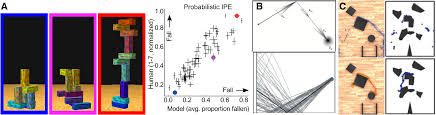
\includegraphics[width=0.62\textwidth]{figs/placeholders/ipe_physics.png}
    % ---------------------------------------------------------------
    \\[-0.2em]
    {\tiny\itshape Placeholder: intuitive physics engine --- probabilistic
     perception predicts ``will it fall?''}
  \end{center}
\end{frame}

% --- Frame 1.1: discrete vs continuous, framed by applications --------
\begin{frame}{Discrete vs.\ continuous}
  The dividing line that matters runs through the \alert{applications}.
  \medskip

  \begin{columns}[T]
    \begin{column}{0.48\textwidth}
      \begin{block}{Discrete}
        Coin flips, Bernoulli / categorical choices, dice.
        \medskip

        Cryptography, differential privacy, randomised algorithms ---
        Applications traditionally within CS - much larger focus.
      \end{block}
    \end{column}
    \begin{column}{0.48\textwidth}
      \begin{block}{Continuous}
        Gaussian noise, sensor models, Bayesian priors over $\mathbb{R}$,
        physical quantities.
        \medskip

        Scientific simulation, Bayesian inference, ML --- where the
        \alert{real-world modelling} happens.
      \end{block}
    \end{column}
  \end{columns}

  \vfill
  \begin{center}
    Continuous distributions are where prior verification work fell short ---\\
    and where this project makes its \wfound{first mechanised} contribution.
  \end{center}
\end{frame}

% --- Frame 1.2: verification is notoriously hard ----------------------
\begin{frame}{Verifying probabilistic programs is notoriously hard}
  \begin{itemize}
    \item Conventional \alert{testing fails}: a rare \emph{correct} outlier
          execution and a genuine bug look \emph{identical}.
    \item Correctness is a property of the whole \alert{distribution}, not of
          any single run.
    \item Reasoning about \alert{independence} and conditioning is subtle and
          error-prone by hand.
  \end{itemize}
  \pause
  \begin{block}{So we need proof}
    Machine-checked, \wfound{foundational} arguments about distributions ---
    resting on nothing but the axioms of mathematics.
  \end{block}
\end{frame}
          % motivation: PP is everywhere
% =====================================================================
%  Contribution frame
%  Central sentence with two hand-drawn-style annotation callouts that
%  pop out on successive overlay clicks.
%    Click 1: base sentence.
%    Click 2: gold arrow out of "mechanisation" -> list (above-left).
%    Click 3: green arrow out of "foundational verification" -> list
%             (above-right).
%  Macros \wmech, \wfound, \wprob and colours wordyellow/green/blue are
%  defined in the main.tex preamble.
% =====================================================================
\begin{frame}{Contribution}
  \vspace*{\fill}
  \vspace*{2.2cm}
  \begin{center}
    \large
    The first \tikzmarknode{mech}{\wmech{mechanisation}}
    of \tikzmarknode{found}{\wfound{foundational verification}}\\[0.5em]
    for \tikzmarknode{prob}{\wprob{probabilistic programs}}\\[0.5em]
    supporting continuous distributions.
  \end{center}
  \vspace*{\fill}
  \begin{tikzpicture}[remember picture, overlay]

    % --- Click 2: gold callout, above-left, out of "mechanisation" ---
    \only<2->{
      \node[anchor=south east, align=left, text width=4.6cm,
            text=wordyellow, font=\small\bfseries] (mechpts)
        at ([xshift=0.0cm, yshift=1.3cm]mech.north) {%
        1.~Soundness proofs\\
        2.~Interactivity using Iris};
      \draw[-{Stealth[length=2.4mm]}, thick, wordyellow]
        (mech.north) to[out=120, in=-70] ([yshift=-1mm]mechpts.south east);
    }
    % --- Click 3: green callout, above-right, out of "foundational
    %     verification" ---
    \only<3->{
      \node[anchor=south west, align=left, text width=5.4cm,
            text=wordgreen, font=\small] (foundpts)
        at ([xshift=-0.4cm, yshift=1.3cm]found.north) {%
        using a theorem prover like Lean or Rocq\\
        Highest achievable assurance\\
        Assuming only the foundational axioms of mathematics};
      \draw[-{Stealth[length=2.4mm]}, thick, wordgreen]
        (found.north) to[out=60, in=-110] ([yshift=-1mm]foundpts.south west);
    }
  \end{tikzpicture}
\end{frame}
         % contribution teaser (arrows)
% --- Background (~5 min): program = distribution -> semantics -> logic ---
% =====================================================================
%  Galton-board slide: a single run vs. the program as a whole.
%
%  Embeds two videos generated by figs/galton_video.py:
%    figs/single.mp4  (95 frames, frame_0 .. frame_94)
%    figs/swarm.mp4   (287 frames, frame_0 .. frame_286)
%
%  Each video is embedded two ways; keep whichever plays in your viewer:
%    (a) multimedia \movie -- a "Screen annotation" pdfpc plays natively.
%        CLICK the poster (frame_0) to play; pdfpc has no autoplay and
%        resets the movie when you leave the slide. Needs GStreamer with
%        an H.264 decoder installed (gstreamer1.0-libav + -plugins-bad).
%    (b) \animategraphics PNG-sequence fallback -- Adobe Reader only.
%  The \animategraphics lines are commented out by default.
%
%  Requires \usepackage{multimedia} and \usepackage{animate} in the
%  preamble (animate is already loaded in main.tex).
% =====================================================================
\begin{frame}{A program is a distribution over runs}

  % ---- Title bar: the type of flip -----------------------------------
  \begin{center}
    $\mathrm{flip} : (m : \mathbb{R}) \to \mathrm{Distrib}\ \{m, m+1\}$
  \end{center}
  \vspace{0.4em}

  \begin{columns}[T]

    % ================= LEFT: single ball =============================
    \begin{column}{0.32\textwidth}
      \centering
      {\small \wprob{an individual ``run'' of the program}}\\[0.3em]

      \movie[loop, showcontrols]%
        {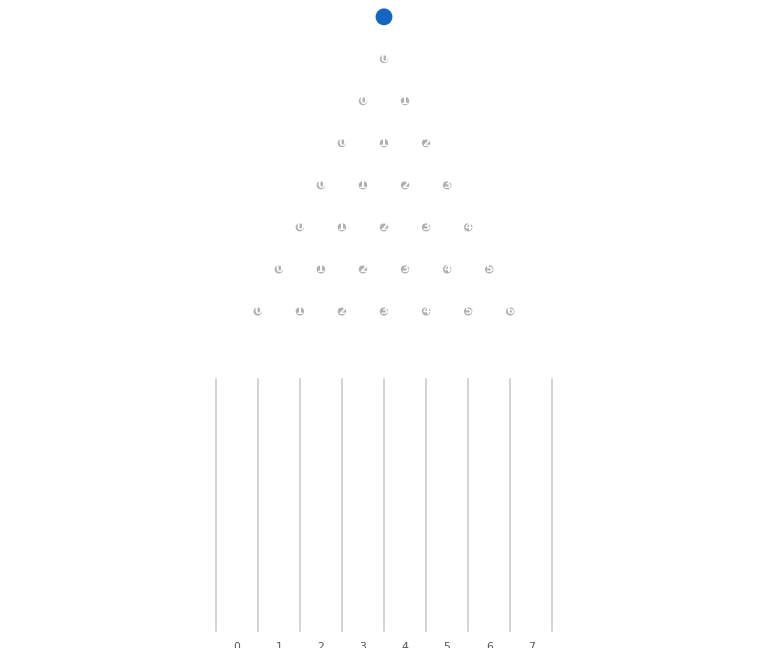
\includegraphics[width=0.92\linewidth]{figs/frame_0.png}}%
        {figs/single.mp4}
      % --- Adobe-Reader-only fallback (comment the \movie above to use) ---
      % \animategraphics[autoplay,loop,width=0.92\linewidth]{25}{figs/single/frame_}{0}{94}

      \vspace{0.3em}

      {\small \wprob{Honing in on a single marble}}
    \end{column}

    % ================= MIDDLE: pseudocode ============================
    \begin{column}{0.34\textwidth}
      \centering
      \vspace{1.6em}
      \[
        \begin{aligned}
          X_0 &\leftarrow \mathrm{flip}\ 0\\
          X_1 &\leftarrow \mathrm{flip}\ X_0\\
          X_2 &\leftarrow \mathrm{flip}\ X_1\\
          \mathrm{ret}&\ X_2
        \end{aligned}
      \]
      \vspace{0.2em}

      {\Large $\mathrel{|\,|\,|}$}
      \vspace{0.4em}

      \[
        \mathrm{for}\ (3,\ \mathrm{flip}\ 0,\ \lambda X.\ \mathrm{flip}\ X)
      \]
    \end{column}

    % ================= RIGHT: swarm ==================================
    \begin{column}{0.32\textwidth}
      \centering
      {\small \wprob{The program as a whole}}\\[0.3em]

      \movie[loop, showcontrols]%
        {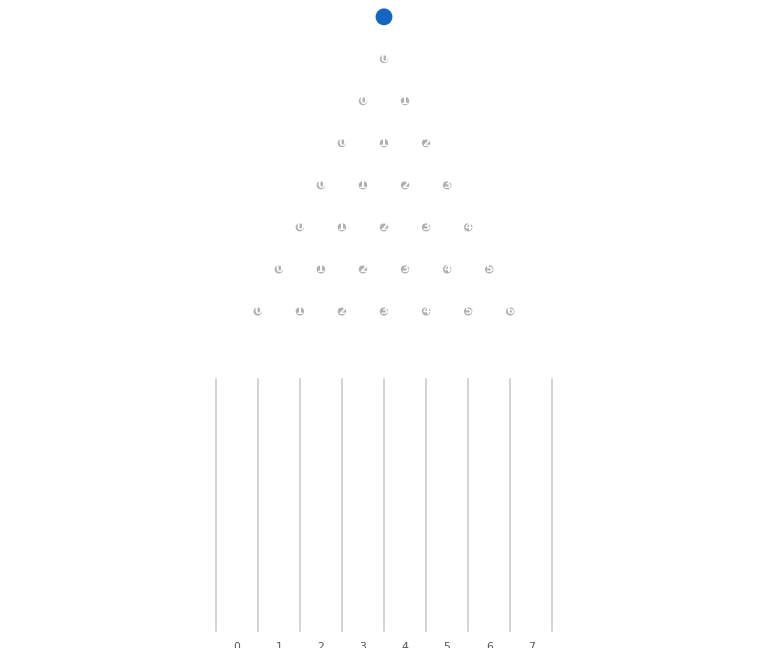
\includegraphics[width=0.92\linewidth]{figs/frame_0.png}}%
        {figs/swarm.mp4}
      % --- Adobe-Reader-only fallback (comment the \movie above to use) ---
      % \animategraphics[autoplay,loop,width=0.92\linewidth]{25}{figs/swarm/frame_}{0}{286}

      \vspace{0.3em}

      {\small \wprob{All the marbles at once}}
    \end{column}

  \end{columns}
\end{frame}
               % a program is a distribution over runs
% =====================================================================
%  Semantics frames (background deck)
%
%  B2 "Probabilistic semantics": the flip program  ≡  its semantics type
%       M : ⟦Γ⟧ → Measure ty
%  B3 "Refining the domain": the SAME type, same on-screen position, but
%     the domain grows by prepending  HC →  giving
%       HC (Hilbert cube) → ⟦Γ⟧ → Measure ty
%
%  DESIGN CHOICE -------------------------------------------------------
%  The "grows into place" effect is realised as a SINGLE frame with beamer
%  overlays (B3 is a continuation of B2 in the same frame). This guarantees
%  the type sits in EXACTLY the same position across overlays: the fixed
%  part  ⟦Γ⟧ → Measure ty  is typeset once and never moves; the  HC →
%  prefix is revealed on the second overlay and fades in via a tikz
%  fading. We anchor the whole expression to the RIGHT of a fixed point so
%  that prepending the prefix grows the formula leftwards into reserved
%  whitespace, leaving the tail (the part the audience tracks) stationary.
%
%  Rather than two separate frames, the single-frame-with-overlays form
%  keeps the layout provably identical (no risk of a 1pt drift between two
%  hand-laid frames) — cleanest continuous animation.
%
%  Macros from main.tex preamble: \sem{·} (⟦·⟧), \alert{}, colour words.
% =====================================================================

% ---------------------------------------------------------------------
%  Frame B2 / B3 — combined, overlay-driven
% ---------------------------------------------------------------------
\begin{frame}{%
    \only<1>{Probabilistic semantics}%
    \only<2->{Refining the domain: the Hilbert cube}%
  }

  \begin{center}
    \begin{minipage}[c]{0.40\textwidth}
      % --- LEFT: the small program, set in plain math (NOT minted) ------
      \centering
      \(
        \begin{aligned}
          X_0 &\leftarrow \mathsf{flip}\ 0\\
          X_1 &\leftarrow \mathsf{flip}\ X_0\\
          X_2 &\leftarrow \mathsf{flip}\ X_1\\
              &\mathsf{ret}\ X_2
        \end{aligned}
      \)
    \end{minipage}%
    \hfill
    \begin{minipage}[c]{0.06\textwidth}
      \centering\Large\(\equiv\)
    \end{minipage}%
    \hfill
    \begin{minipage}[c]{0.52\textwidth}
      % --- RIGHT: the semantics TYPE, large and prominent ---------------
      % The expression is right-anchored: the fixed tail never moves; the
      % HC → prefix grows leftwards into reserved whitespace.
      %
      % KEY trick: the prefix "HC →" RESERVES its full width on EVERY
      % overlay via a \phantom, so the fixed tail (⟦Γ⟧ → Measure ty) never
      % moves. The visible glyphs are overprinted in the same zero-extra-
      % width box (\rlap) and revealed only on overlay 2+, so the prefix
      % "grows into place" while the tail stays pinned in position.
      \raggedleft
      \Large
      \(
        M : {}
        \rlap{\(\only<2->{\alert{\mathrm{HC}}\;\alert{\to}}\)}%
        \phantom{\mathrm{HC}\;\to}\;
        % --- the FIXED tail: typeset once, identical on every overlay ----
        \sem{\Gamma} \to \mathrm{Measure}\ \mathit{ty}
      \)
      % --- small annotation under the HC prefix (overlay 2+) ------------
      \\[0.2em]
      \only<2->{\makebox[\linewidth][l]{\hspace*{0.2cm}%
        \alert{\footnotesize \(\mathrm{HC}\) = Hilbert cube \(=[0,1]^{\mathbb{N}}\)}}}
    \end{minipage}
  \end{center}

  \vfill

  % -------------------------------------------------------------------
  %  Stylised Hilbert-cube illustration (overlay 2+).
  %  A row of ~6 coordinate cells: scattered sample dots, a couple
  %  crossed out, thin curved arrows into a {X₁, X₂, X₃} label.
  % -------------------------------------------------------------------
  % stylised placeholder — swap for a nicer asset later
  \only<2->{%
  \begin{center}
  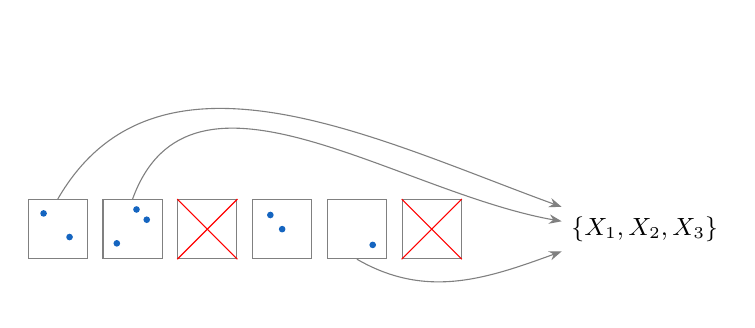
\begin{tikzpicture}[
      cell/.style={draw, gray, thin, minimum size=0.75cm, inner sep=0pt},
      dot/.style={circle, fill=wordblue, inner sep=0pt, minimum size=2.4pt},
      arr/.style={-{Stealth[length=1.6mm]}, thin, gray},
    ]
    % --- the coordinate cells -----------------------------------------
    \foreach \i in {0,...,5} {
      \node[cell] (c\i) at (\i*0.95,0) {};
    }
    % --- scattered sample dots inside a few cells ---------------------
    \node[dot] at ([shift={(-0.18, 0.20)}]c0.center) {};
    \node[dot] at ([shift={( 0.15,-0.10)}]c0.center) {};
    \node[dot] at ([shift={( 0.05, 0.25)}]c1.center) {};
    \node[dot] at ([shift={(-0.20,-0.18)}]c1.center) {};
    \node[dot] at ([shift={( 0.18, 0.12)}]c1.center) {};
    \node[dot] at ([shift={( 0.00, 0.00)}]c3.center) {};
    \node[dot] at ([shift={(-0.15, 0.18)}]c3.center) {};
    \node[dot] at ([shift={( 0.20,-0.20)}]c4.center) {};
    % --- a couple of cells crossed out (✗) ----------------------------
    \draw[red, thin] (c2.south west) -- (c2.north east);
    \draw[red, thin] (c2.north west) -- (c2.south east);
    \draw[red, thin] (c5.south west) -- (c5.north east);
    \draw[red, thin] (c5.north west) -- (c5.south east);
    % --- label to the right -------------------------------------------
    \node[anchor=west, font=\small] (lbl) at (6.4,0)
      {\(\{X_1, X_2, X_3\}\)};
    % --- thin arrows curving from active cells into the label ---------
    \draw[arr] (c0.north) to[out=60, in=160] (lbl.north west);
    \draw[arr] (c1.north) to[out=70, in=170] ([yshift=1mm]lbl.west);
    \draw[arr] (c4.south) to[out=-30, in=200] (lbl.south west);
  \end{tikzpicture}
  \end{center}%
  }
\end{frame}
            % M : ⟦Γ⟧ → Measure ty, then HC domain
% =====================================================================
%  Background frame: how to verify -- probabilistic separation logic
%  Single-variable `unif1` example throughout (X ← unif[0,1]; ret X).
%
%  Animates in three beats:
%    Beat 1: program  ≡  awful integral denotation.
%    Beat 2: big red ✗ strikes through the integral (we do NOT compute it).
%    Beat 3: the separation-logic alternative -- reason directly about
%            the variable, X ∼ unif[0,1], with a blue hand-drawn note and
%            a curved arrow from the crossed-out integral to the assertion.
%
%  Macros \wprob and colours wordblue defined in main.tex preamble.
% =====================================================================
\begin{frame}{How to verify: probabilistic separation logic}
  \begin{center}
    % --- Beat 1: program  ≡  denotation ---------------------------------
    \large
    $\underbrace{X \leftarrow \mathrm{unif}[0,1];\ \ \mathrm{ret}\ X}_{\text{\normalsize program}}$

    \smallskip
    $\equiv$
    \smallskip

    \tikzmarknode{intl}{}%
    $\underbrace{%
      \lambda E \mapsto \int (\lambda \mu \mapsto \mu\,E)\;
        d\bigl(\mathrm{map}\,(\lambda X \mapsto \mathrm{dirac}\,X)\;\mathrm{unif}[0,1]\bigr)
    }_{\text{\normalsize denotation}}$%
    \tikzmarknode{intr}{}
  \end{center}

  \vspace*{0.3cm}

  % --- Beat 3: the separation-logic alternative ----------------------
  \onslide<3->{%
    \begin{center}
      \large
      \wprob{reason directly about the variables}\\[0.5em]
      \tikzmarknode{simassert}{}%
      {\Large $X \sim \mathrm{unif}[0,1]$}
    \end{center}
  }

  \begin{tikzpicture}[remember picture, overlay]
    % --- Beat 2: red strike-through across the integral expression ----
    \onslide<2->{
      \draw[red, line width=2pt]
        ([yshift=3.5mm]intl.north east) -- ([yshift=-3.5mm]intr.south west);
      \draw[red, line width=2pt]
        ([yshift=-3.5mm]intl.south east) -- ([yshift=3.5mm]intr.north west);
    }

    % --- Beat 3: curved blue arrow from crossed integral to assertion -
    \onslide<3->{
      \draw[-{Stealth[length=2.8mm]}, line width=1pt, wordblue]
        ([yshift=-5mm]$ (intl)!0.5!(intr) $)
          to[out=-90, in=150]
        ([xshift=-4mm, yshift=1mm]simassert.west);
    }
  \end{tikzpicture}
\end{frame}
       % how to verify: separation logic (unif1)
% =====================================================================
%  Background: Iris and the logic of bunched implications (BI)
%  \input-able frame(s) only; no preamble. See main.tex for macros.
% =====================================================================

\begin{frame}{Iris, and the logic of bunched implications (BI)}
  The separation logic is built on the Lean port of \alert{Iris}; its
  assertions \(\mathrm{Prop}\) form a \wmech{BI (bunched-implication) logic}.
  \vfill
  % --- The assertion-language signature -------------------------------
  \begin{center}
  \renewcommand{\arraystretch}{1.35}
  \(
    \begin{array}{r@{\;\;}c@{\;\;}l@{\qquad}l}
      \ulcorner\,\cdot\,\urcorner
        & : & \mathrm{Prop} \to \mathrm{Prop}
        & \text{\footnotesize pure embedding} \\
      \mathsf{True},\ \mathsf{False},\ \mathsf{emp}
        & : & \mathrm{Prop}
        & \text{\footnotesize units} \\
      \wedge,\ \vee,\ \Rightarrow,\ \wprob{\ensuremath{\ast}},\ \wprob{\ensuremath{\wand}}
        & : & \mathrm{Prop} \times \mathrm{Prop} \to \mathrm{Prop}
        & \text{\footnotesize binary connectives} \\
      \forall,\ \exists
        & : & \forall A.\ (A \to \mathrm{Prop}) \to \mathrm{Prop}
        & \text{\footnotesize quantifiers}
    \end{array}
  \)
  \end{center}
  \vfill
  \begin{flushright}\footnotesize
    \wprob{\(\ast\)} separating conjunction \quad
    \wprob{\(\wand\)} magic wand \quad
    --- the separation-logic-specific connectives.
  \end{flushright}
\end{frame}


\begin{frame}{Iris, and the logic of bunched implications (BI)}
  Assertions \(\mathrm{Prop}\) form a \wmech{BI (bunched-implication) logic} on
  the Lean port of \alert{Iris}.
  \smallskip
  % --- The assertion-language signature -------------------------------
  \begin{center}
  \renewcommand{\arraystretch}{1.2}
  \(
    \begin{array}{r@{\;\;}c@{\;\;}l@{\qquad}l}
      \ulcorner\,\cdot\,\urcorner
        & : & \mathrm{Prop} \to \mathrm{Prop}
        & \text{\footnotesize pure embedding} \\
      \mathsf{True},\ \mathsf{False},\ \mathsf{emp}
        & : & \mathrm{Prop}
        & \text{\footnotesize units} \\
      \wedge,\ \vee,\ \Rightarrow,\ \wprob{\ensuremath{\ast}},\ \wprob{\ensuremath{\wand}}
        & : & \mathrm{Prop} \times \mathrm{Prop} \to \mathrm{Prop}
        & \text{\footnotesize binary connectives} \\
      \forall,\ \exists
        & : & \forall A.\ (A \to \mathrm{Prop}) \to \mathrm{Prop}
        & \text{\footnotesize quantifiers}
    \end{array}
  \)
  \end{center}
  \smallskip
  \begin{itemize}
    \item<2->
      \alert{A logic inside a logic.} \(\mathrm{Prop}\) is an object logic
      inside Lean's meta-logic.\footnote<3->{Revisited later in the talk.}
    \item<3->
      \alert{Impredicativity.} \(\forall/\exists\) range over an
      \emph{arbitrary} type \(A\) --- including \(\mathrm{Prop}\) itself: we
      may quantify over propositions.
  \end{itemize}
\end{frame}
              % Iris & the BI definition
% --- Contribution, precisely + formalisation dependency graph -----------
% =====================================================================
%  Contributions, revisited --- the mechanisation of Lilac
%  \input-able frames only; no preamble. See main.tex for macros.
% =====================================================================

\begin{frame}{Contributions, ``revised''}
  Now that the motivation is in place: \alert{what} did we mechanise, and
  \alert{why} does it matter?
  \vfill
  \begin{itemize}
    \item \wprob{Lilac} is a probabilistic separation logic whose guiding
          idea is\\[0.2em]
          \begin{center}
            \emph{``separation \(=\) independence of random variables''}
          \end{center}
          The separating conjunction \(P * Q\) asserts that the random
          variables described by \(P\) and \(Q\) are \alert{probabilistically
          independent} --- and Lilac supports \wprob{continuous} distributions.
    \item We give the \wmech{first mechanisation of \textbf{Core\footnote{Extended Lilac adds reasoning about conditioning} Lilac} in Lean 4},
          the first mechanisation of \emph{any} probabilistic separation logic
          in Lean.
  \end{itemize}
\end{frame}


\begin{frame}{What was mechanised}
  \begin{itemize}
    \item[\textcolor{wordyellow}{\textbf{1.}}]
          \wfound{Soundness, from the ground up.}
          Core Lilac is built as a model over probability spaces with finite
          footprint, and every program-logic proof rule is proved sound
          against that model:
          \[
            \texttt{wp\_ret}\quad
            \texttt{wp\_bind}\quad
            \texttt{wp\_unif}\quad
            \texttt{wp\_cons}\quad
            \texttt{wp\_frame}
          \]
    \pause
    \item[\textcolor{wordyellow}{\textbf{2.}}]
          \wfound{An interactive proof interface.}
          Lilac is instantiated as a \wmech{bunched-implication logic} on the
          Lean port of \alert{Iris}, so proofs are carried out in the
          \emph{Iris proof mode}.
    \pause
    \item[\textcolor{wordyellow}{\textbf{3.}}]
          \wfound{Worked examples.}
          Specifications of sampling programs proved in that proof mode ---
          including constructing a \alert{separating conjunct of two
          independent uniform samples}.
  \end{itemize}
\end{frame}



% --- Closing ----------------------------------------------------------
% \begin{frame}[standout]
%   Thank you!\\[1em]
%   \small Questions?
% \end{frame}

\end{document}
